\section{研究现状}
随着量子计算硬件规模的快速增长,量子电路的验证成为一个重要问题。开始的研究主要集中在BDD在量子计算下的推广算法,如量子信息决策图(Quantum Information Decision Diagram,或QuIDD)\citep{Viamontes_2003},量子多值决策图(Quantum multiple-valued Decision Diagram,或QMDD)\citep{Seiter_2013}等,从而对组合式量子电路进行等效性检查。显然,随着越来越复杂的物理可实现化的硬件出现,将会出现更加复杂的,更加针对于的,新的验证问题。比如量子存储\citep{Kerckhoff_2010},量子反馈网络\citep{Gough_2008},RUS量子电路\citep{Bocharov_2015}。量子模型检测可以为量子电路的验证提供了更多思路。

量子系统模型检测的早期工作旨在验证量子通信协议\citep{Gay,BALTAZAR_2008,davidson2012model}。后来还有针对分析和验证量子程序的应用\citep{ying2016foundations},比如量子自动机\citep{ying2014model}、量子马尔可夫链\citep{Ying_2013}和超算符值马尔可夫链\citep{feng2013model}的模型检测技术。然而,在这些量子模型检测技术与它们在验证量子电路方面实际应用之间存在巨大差距仍需填补。TDD作为新的数据结构,极大加快了计算过程,有可能深化二者的联系,加快实际应用的出现。

在本节中,将探讨本研究的核心内容,即“量子模型检测中的时序逻辑的验证”。
这一研究问题在量子计算领域具有重要的理论与实际意义,关乎量子计算机的精确性和效率。为了解决这一问题,本研究采用了方法论为利用TDD(Tensor Decision Diagram)数据结构来快速模拟量子计算过程。这种方法提高了计算效率,为量子计算提供了更加准确的模拟。

进一步地,研究过程中将探讨四种可能的优化途径,这些途径旨在进一步提升模拟过程的效率。
这四种方法既有来源于经典计算机的思路,也有量子计算机特有的思路。每一种方法都将简要说明。


\subsection{研究方法}
本次研究的主要目的是借助TDD数据结构,构建能快速计算量子模型检测中可达问题的方案。因此主要采用的方法是模拟量子计算。本次研究的主要挑战在于尽可能减少程序的运行时间。为此,需要采用一系列方法来开发更有效的算法,以优化TDD操作和收缩张量网络。其中包括开发新技术来分割张量网络和优化TDD结构。
下面简单介绍以下具体研究方法。

\begin{myen}

\item \label{addition}关于常用的量子线路划分方法,
第一种被称为addition\citep{chen2018classical}。将量子电路视为张量网络,首先将一个量子电路C转换成无向图G。G中的每个节点表示量子电路的一个索引,并且如果它们是相同门的输入或输出索引,则在G中连接两个节点。并且当满足以下两个条件之一时输入和输出索引不变:
\begin{itemize}
	\item 是对角线量子门的输入和输出索引;
	\item 是受控门的控制比特位的输入和输出索引。
\end{itemize}
	
图\ref{fig:addition}展示了Grover\_3电路图的索引链接图。该图描述了量子电路的连通性,通过选择图中连通度最大的索引可以对电路进行分割。因此选择图中连通度较大的$x_1^1,x_1^3x_2^1$可以对电路进行较好的划分。
 
\begin{figure}[!htbp]
	\centering
	\includegraphics[height=5cm]{Img/cir_index_graph.pdf}
	\caption{Grover\_3的索引连接图}
	\label{fig:addition}
\end{figure} 

\item 另一种常用的电路划分方法成为contraction。在这一方法中,将量子电路划分为若干个较小的部分,其收缩等于原始电路。对于两个预设整数参数k1和k2,将电路划分为若干小电路。其中每个小电路涉及最多k1个量子比特,并且与至多跨越不同部件的k2个多比特门相连。图\ref{fig:contraction}展示了对Bit flip电路进行k1=3,k2=2的拆分结果。
\begin{figure}[!htbp]
	\centering
	\includegraphics[height=4.5cm]{Img/cir_contraction.pdf}
	\caption{对Bit flip电路进行contraction的拆分}
	\label{fig:contraction}
\end{figure} 


\item \label{contraction}在BDD中,索引的顺序很重要。因为索引顺序会直接影响BDD的大小。一个良好的变量顺序可以使得BDD比一个糟糕的变量顺序小得多。图\ref{fig:bdd-compare}的了两张图都表示了布尔函数ƒ(x1,...,x8)=x1x2+x3x4+x5x6+x7x8,但图\ref{fig:bdd-good}的结构更简单。其中图\ref{fig:bdd-bad}的索引顺序为\{x1,x3,x5,x7,x2,x4,x6,x8\},图\ref{fig:bdd-good}的索引顺序为\{x1,x2,x3,x4,x5,x6,x7,x8\}。找到一个好的索引顺序是一个NP问题。在工程实现中,目前只能通过小规模电路上寻求规律,然后在更大规模电路中应用较优顺序。

\begin{figure}[!htbp]
	\centering
	\begin{subfigure}[b]{.4\textwidth}
        \centering
        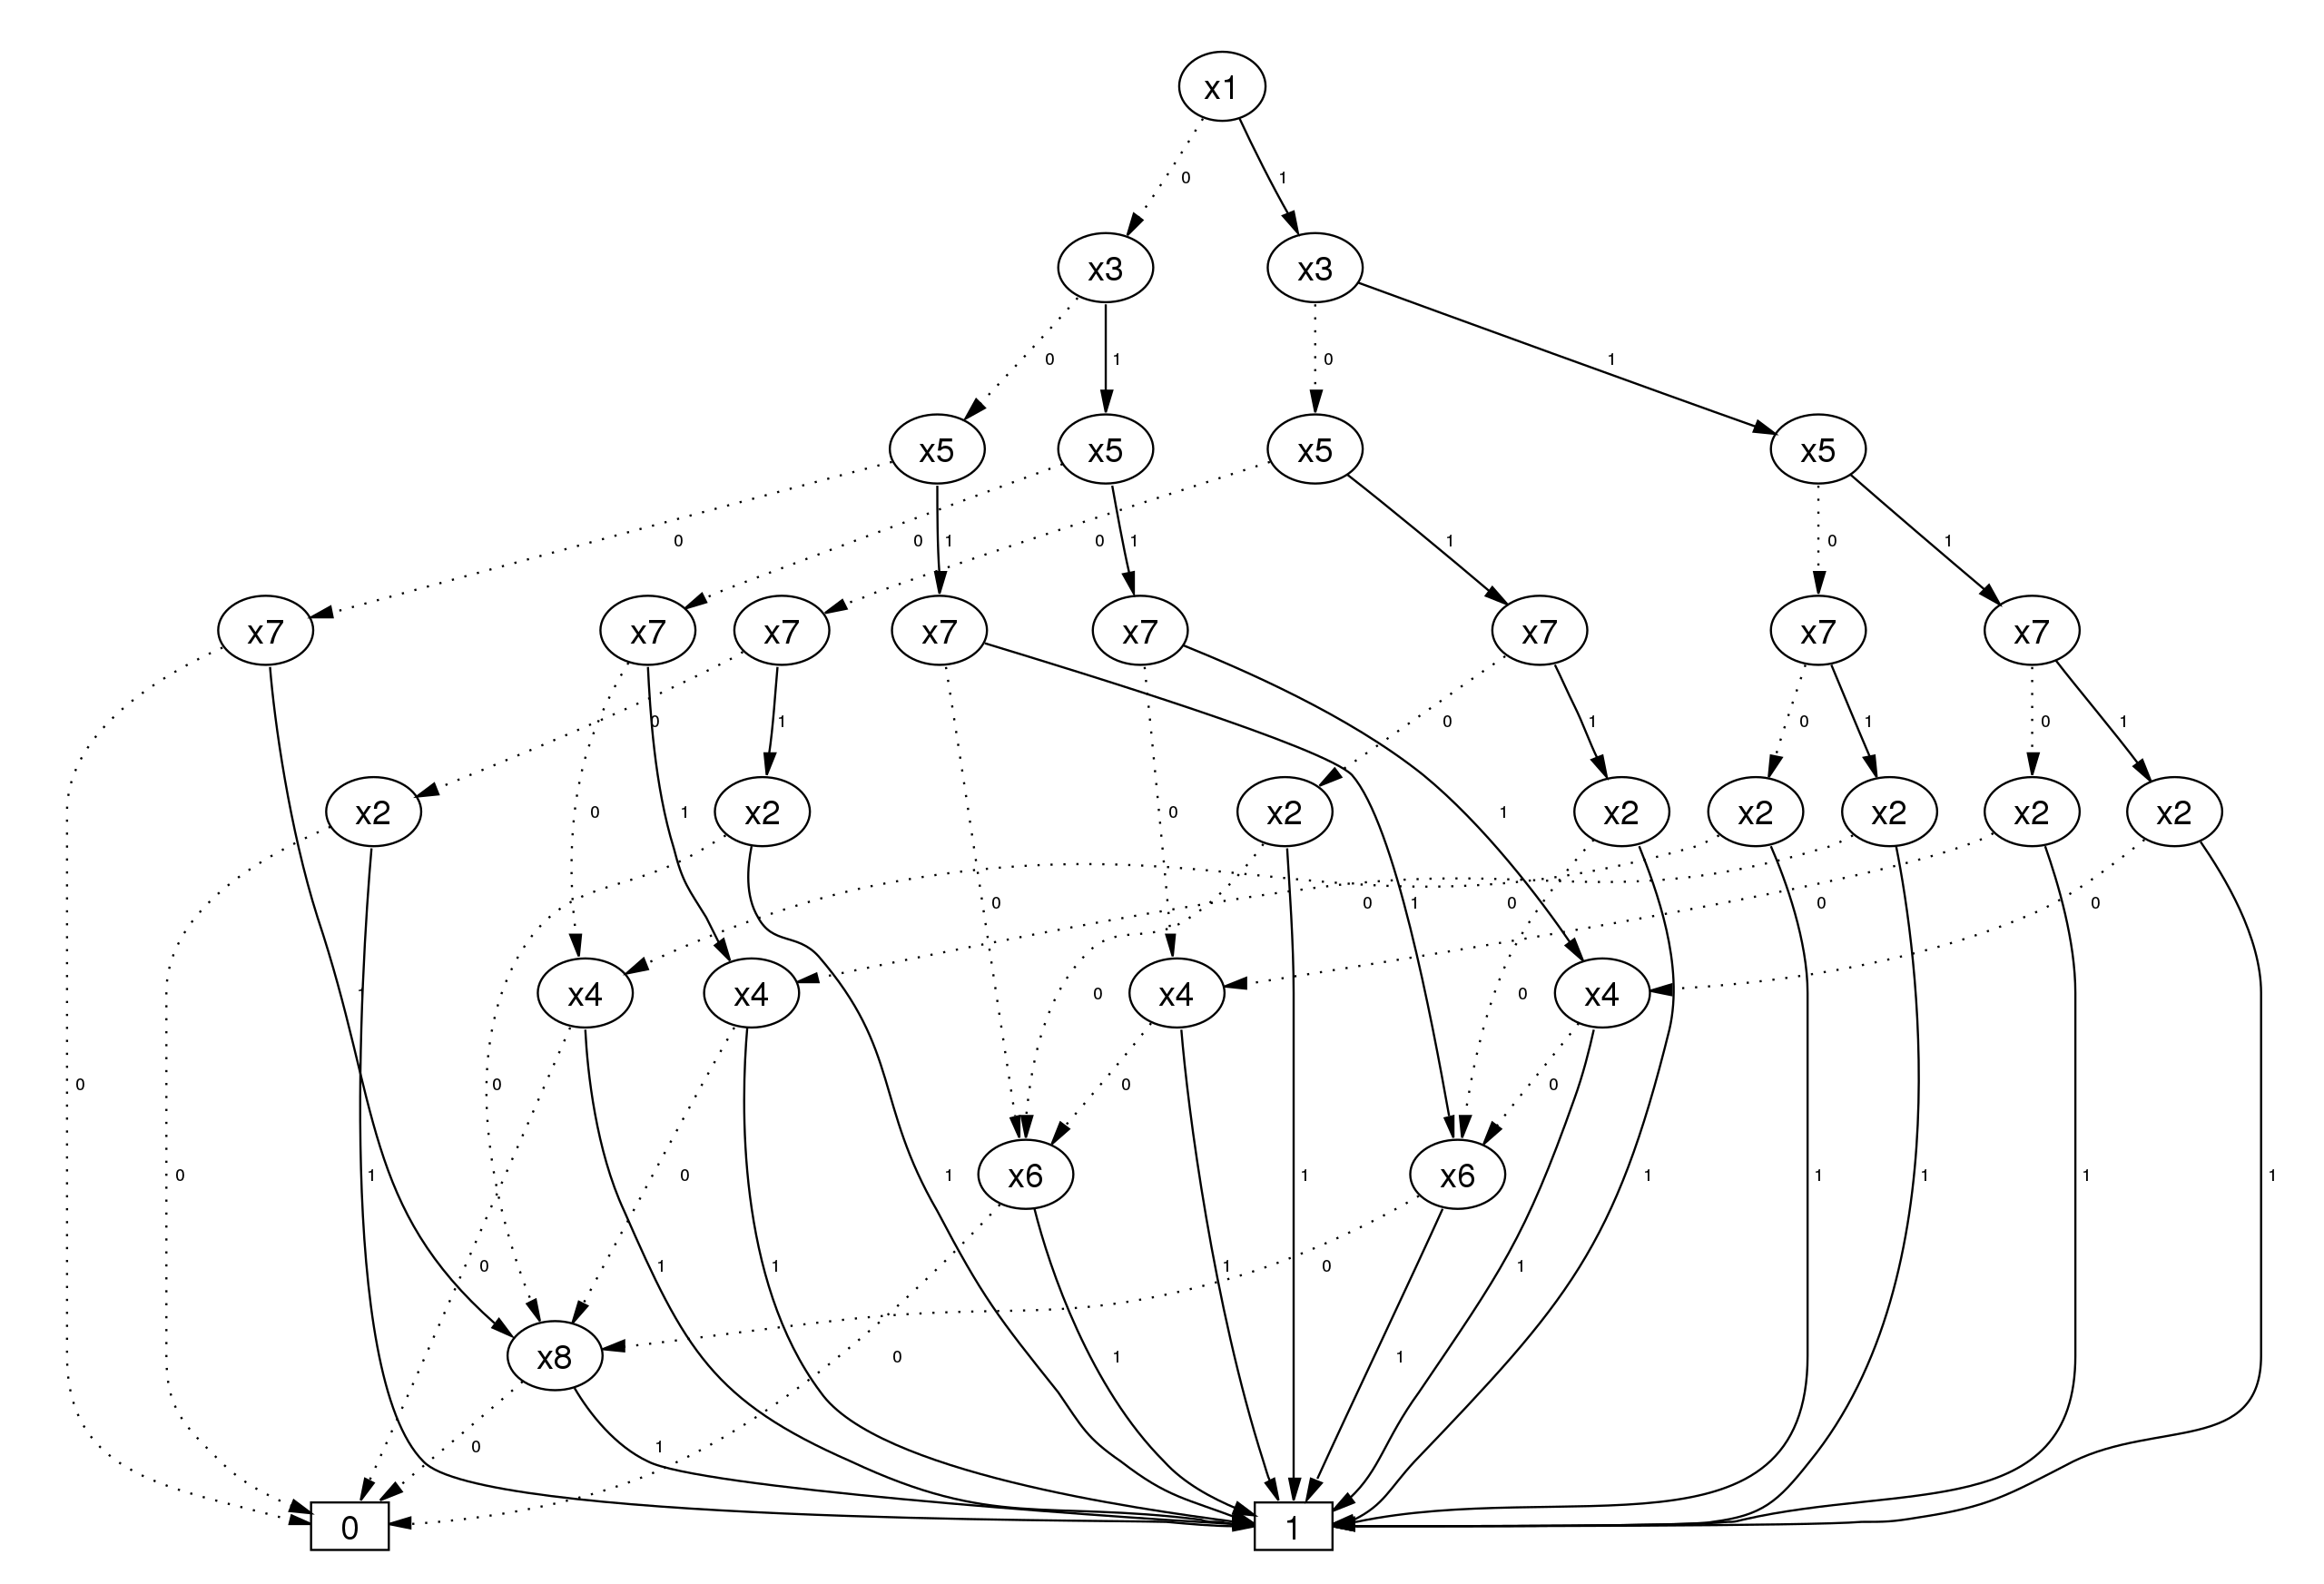
\includegraphics[height=4.5cm]{Img/BDD_Variable_Ordering_Bad.svg.pdf}
		\caption{索引顺序为\{x1,x3,x5,x7,x2,x4,x6,x8\}}
		\label{fig:bdd-bad}
	\end{subfigure}
	\begin{subfigure}[b]{.4\textwidth}
        \centering
        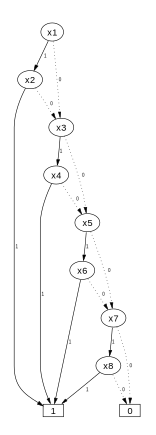
\includegraphics[height=5cm]{Img/BDD_Variable_Ordering_Good.svg.pdf}
		\caption{索引顺序为\{x1,x2,x3,x4,x5,x6,x7,x8\}}
		\label{fig:bdd-good}
	\end{subfigure}
	\caption{同一布尔函数在不同索引顺序下的结构图\citep{wiki:bdd}}
	\label{fig:bdd-compare}
\end{figure}


\item 由于量子状态都在同一希尔伯特空间中。因此作用某些算子后,不同的量子状态可能等价。
当存储算子的资源少于存储状态的资源时,就有可能存储算子表示不同的状态\citep{vinkhuijzen2023limdd}。图\ref{fig:qmdd-example}表示了一个QMDD的例子,应用等价性,可以化简为图\ref{fig:limdd-example}。
TDD也可以应用类似技术,进行进一步化简,从而降低资源要求。
\begin{figure}[!htbp]
    \centering
    \begin{subfigure}[b]{.4\textwidth}
        \centering
        \includegraphics[height=6cm]{Img/limdd.pdf}
        \caption{一个QMDD示例}
        \label{fig:qmdd-example}
    \end{subfigure}
    \begin{subfigure}[b]{.4\textwidth}
        \centering
        \includegraphics[height=6cm]{Img/limdd_reduce.pdf}
        \caption{应用等价性化简图\ref{fig:qmdd-example}}
        \label{fig:limdd-example}
    \end{subfigure}
\end{figure}
\end{myen}
\subsection{存在的问题}
在本研究过程中,主要遇到了两个问题,这些问题对研究的深入发展和实际应用产生了重要影响。

首先,面临的一个关键挑战是如何将所提出的方法扩展应用到更大规模的实例。这不仅涉及到算法的效率问题,还包括数据处理能力的提升。对于实现验证量子计算算法在更广泛领域的应用至关重要。为了解决这一挑战,目前采用电路拆分方法来降低TDD的资源消耗,并挖掘可能的并行计算机会。此外,还计划应用更灵活的索引策略和limdd的思路,以期达到更高效的处理效果。

其次,另一个重要的问题是如何将研究方法应用于更加实用的示例。这是将理论研究转化为实际应用的关键一步。目前考虑的主要方向是将此方法应用到量子线路设计,即QDA(Quantum Design Automation)领域。
计划未来能够将本研究成果应用于不同的synthesis算法的验证等价性中,从而在量子计算的实际应用中发挥更大的作用。
